\section{Illumination model}
\label{sec:illum}
\here{8}
The local illumination model sums an ambient term, and for every light a diffuse (Lambert) and a
specular (Blinn--Phong) term, scaled by the light's attenuation and, for a spot light, its cone factor.
\begin{equation}
I = k_a I_a + \sum_{l} f_{\text{att},l}\,c_l\,I_l\Big[k_d\,\max(0,\vect N\cdot\vect L_l) + k_s\,\max(0,\vect N\cdot\vect H_l)^{n}\Big],
\qquad \vect H=\frac{\vect L+\vect V}{\lVert\vect L+\vect V\rVert}
\label{eq:phong}
\end{equation}
\begin{equation}
f_{\text{att}}=\frac{1}{1+k_l d+k_q d^2},\qquad
c_{\text{spot}}=\Big(\mathrm{clamp}\Big(\frac{\cos\gamma-\cos\theta_o}{\cos\theta_i-\cos\theta_o},0,1\Big)\Big)^2
\label{eq:att}
\end{equation}
\textbf{Phong and Blinn--Phong.} Both specular terms are standard; the code uses the half-vector form.
\begin{gather}
\text{Phong: } I_s=k_s\max(0,\vect R\cdot\vect V)^n,\qquad \vect R=2(\vect N\cdot\vect L)\vect N-\vect L\label{eq:phongblinn}\\
\text{Blinn--Phong (used): } I_s=k_s\max(0,\vect N\cdot\vect H)^n,\qquad \vect H=\frac{\vect L+\vect V}{\lVert\vect L+\vect V\rVert}\nonumber
\end{gather}
\begin{itemize}
\item The angle between $\vect N$ and $\vect H$ is half the angle between $\vect R$ and $\vect V$, so the Blinn lobe of exponent
$n$ is wider; $(\vect N\cdot\vect H)^{4n}\approx(\vect R\cdot\vect V)^{n}$ (Figure~\ref{fig:phongblinn}a).
\item $\vect H$ needs no reflection vector and stays defined when $\vect V$ is below the surface's tangent plane.
\end{itemize}
\textbf{As implemented} (\code{rendering/ShaderSources.cpp: computeLight, brdf, compose}). The colour of a surface point is
\begin{gather}
\vect c=\boldsymbol\rho\odot\Big(\vect E_{\text{amb}}\,a+\sum_l v_l\,\vect E_l\max(0,\vect N\cdot\vect L_l)\Big)
+\sum_l v_l\,\vect E_l\,k_s\max(0,\vect N\cdot\vect H_l)^n+\boldsymbol\rho\,e\label{eq:illumcode}\\
\vect E_l=I_l\,\vect c_l\,f_{\text{att},l}\,c_{\text{spot},l}\nonumber\\
\text{lamps: } f_{\text{att}}=\frac{\operatorname{clamp}\big(1-(d/r)^4\big)^2}{1+d^2},\qquad
c_{\text{cone}}=\operatorname{smoothstep}\big(\cos\theta_c,\ \cos\theta_c+0.1,\ -\vect L\cdot\vect a\big)\label{eq:lampatt}
\end{gather}
\begin{itemize}
\item $\boldsymbol\rho$: the part's base colour converted to linear ($\boldsymbol\rho=\vect c_{\text{base}}^{2.2}$, so $k_a=k_d=\boldsymbol\rho$);
$a$: ambient occlusion (Section~\ref{sec:post}); $v_l$: shadow visibility of the key light and the shadowed searchlight
(Eq.~\eqref{eq:shadow}), 1 for the others; $e$: emission of lamps and screens.
\item $\vect E_{\text{amb}}$ is the hemisphere / spherical-harmonic sky irradiance of Table~\ref{tab:lights}, not a constant.
\item The lamps' window $(1-(d/r)^4)^2$ brings the inverse-square falloff to exactly zero at the range $r$
(3.5--26\,m), so at most 16 lamps per fragment are needed (Figure~\ref{fig:atten}b).
\end{itemize}
\begin{lstlisting}[language=C++,caption={The per-light reflectance, Blinn--Phong and Cook--Torrance (\code{src/rendering/ShaderSources.cpp: brdf}, GLSL).}]
void brdf(vec3 N, vec3 V, vec3 L, vec3 radiance, vec3 F0, float rough, out vec3 diff, out vec3 spec) {
    diff = vec3(0.0);  spec = vec3(0.0);
    float nl = max(dot(N, L), 0.0);
    if (nl <= 0.0) return;
    vec3 H = normalize(L + V);
    if (uPbr == 0) {  // Blinn-Phong: k_d (N.L) + k_s (N.H)^n
        diff = radiance * nl;
        spec = radiance * uSpecular * pow(max(dot(N, H), 0.0), uShininess);
        return;
    }
    // Cook-Torrance: D (GGX) * G (Smith-Schlick) * F (Schlick) / (4 N.V N.L)
    float nv = max(dot(N, V), 1e-3), nh = max(dot(N, H), 0.0), vh = max(dot(V, H), 0.0);
    float a = rough * rough, a2 = a * a;
    float dd = nh * nh * (a2 - 1.0) + 1.0;
    float D = a2 / (PI * dd * dd);
    float k = (rough + 1.0) * (rough + 1.0) / 8.0;
    float G = (nv / (nv * (1.0 - k) + k)) * (nl / (nl * (1.0 - k) + k));
    vec3 F = F0 + (1.0 - F0) * pow(1.0 - vh, 5.0);
    spec = radiance * nl * PI * D * G * F / (4.0 * nv * nl);
    diff = radiance * nl * (1.0 - F) * (1.0 - uMetalness);
}
\end{lstlisting}
\begin{gather}
f_s=\frac{D\,G\,F}{4(\vect N\cdot\vect V)(\vect N\cdot\vect L)},\qquad
D=\frac{\alpha^2}{\pi\big((\vect N\cdot\vect H)^2(\alpha^2-1)+1\big)^2},\quad \alpha=r^2\label{eq:ggx}\\
G=\prod_{\vect x\in\{\vect V,\vect L\}}\frac{\vect N\cdot\vect x}{(\vect N\cdot\vect x)(1-k)+k},\quad k=\frac{(r+1)^2}{8}\nonumber\\
F=F_0+(1-F_0)(1-\vect V\cdot\vect H)^5,\quad F_0=\operatorname{mix}(0.04,\boldsymbol\rho,m),\qquad
\text{diffuse}=(1-F)(1-m)\,\boldsymbol\rho\max(0,\vect N\cdot\vect L)\nonumber
\end{gather}
with roughness $r$ and metalness $m$ per part. The Trowbridge--Reitz microfacet distribution (GGX) lobe replaces $(\vect N\cdot\vect H)^n$ and keeps energy balanced
between diffuse and specular (Figure~\ref{fig:phongblinn}b, Figure~\ref{fig:materials}).
\begin{figure}[htbp]
\centering\plot{p_phong_blinn}{\linewidth}
\caption{(a) Phong and Blinn--Phong lobes for the same exponent as the view sweeps past the mirror direction
(Eq.~\eqref{eq:phongblinn}); (b) the GGX distribution $D$ of Eq.~\eqref{eq:ggx} for three roughness values against a
Blinn lobe, each divided by its peak.}
\label{fig:phongblinn}
\end{figure}
\begin{figure}[htbp]
\centering\plot{p_attenuation}{\linewidth}
\caption{Light falloff with the code's constants: (a) the beacon and searchlight attenuation of Eq.~\eqref{eq:att};
(b) the windowed lamp falloff of Eq.~\eqref{eq:lampatt} for three lamp ranges; (c) the searchlight's soft cone
(Eq.~\eqref{eq:att}) and the hooded lamps' cone (Eq.~\eqref{eq:lampatt}).}
\label{fig:atten}
\end{figure}
\begin{figure}[htbp]
\centering
\raw{lab/materials_blinnphong_row}{0.92\linewidth}\\[1.5mm]
\raw{lab/materials_pbr_grid}{0.62\linewidth}
\caption{The two reflectance models as the renderer draws them on spheres. Top: Blinn--Phong ($k_s=0.6$) with
$n=4,16,64,256$: the highlight shrinks as $n$ grows. Bottom: GGX / Cook--Torrance, roughness across, metalness down,
under the moon and one warm point lamp.}
\label{fig:materials}
\end{figure}
\begin{table}[htbp]
\caption{The illumination equations and the code that evaluates them (GLSL in \code{rendering/ShaderSources.cpp}).}\label{tab:illumcode}
\centering\small
\begin{tabularx}{\linewidth}{@{}>{\raggedright\arraybackslash}p{3.2cm}>{\raggedright\arraybackslash}p{3.6cm}X@{}}
\toprule
Term & Equation & Code (exact line)\\\midrule
Lambert diffuse & $\max(0,\vect N\cdot\vect L)$ & \code{float nl = max(dot(N, L), 0.0); diff = radiance * nl;}\\
Blinn--Phong specular & Eq.~\eqref{eq:phongblinn} & \code{spec = radiance * uSpecular * pow(max(dot(N, H), 0.0), uShininess);}\\
Point / spot attenuation & Eq.~\eqref{eq:att} & \code{rad = uBeaconColor / (1.0 + uBeaconAtt.x * dist + uBeaconAtt.y * dist * dist);}\\
Spot cone & Eq.~\eqref{eq:att} & \code{cone = clamp((dot(-L, uSpotDir) - uSpotCos.y) / (uSpotCos.x - uSpotCos.y), 0, 1); rad *= cone * cone}\\
Lamp falloff & Eq.~\eqref{eq:lampatt} & \code{att = window * window / (1.0 + dist * dist);} (\code{practicalAttenuation})\\
GGX, Smith, Schlick & Eq.~\eqref{eq:ggx} & \code{brdf()} when \code{uPbr == 1}\\
Sum of the terms & Eq.~\eqref{eq:illumcode} & \code{compose()}: \code{albedo * diffuse + specular + albedo * uEmissive}\\
\bottomrule
\end{tabularx}
\end{table}

\begin{table}[htbp]
\caption{Light sources.}\label{tab:lights}
\centering\small
\begin{tabularx}{\linewidth}{@{}llXl@{}}
\toprule
Light & Type & Parameters & When\\\midrule
Sun & directional & direction and colour from the solar model (Section~\ref{sec:day}), intensity up to 3.2 & sun above $-1^\circ$\\
Moon & directional & intensity \moonI, colour (0.55, 0.62, 0.80) & night\\
Beacon & point & $k_l=\beaconLin$, $k_q=\beaconQuad$, pulsing 0.6--2.0 & night\\
UAV searchlight & spot & $\theta_i=\spotInner^\circ$, $\theta_o=\spotOuter^\circ$, $k_l=\spotLin$, $k_q=\spotQuad$ & night, UAV airborne\\
Practical lamps & point & up to 16 at once (floodlights, lamps, fire barrel) & dusk to dawn\\
Ambient & hemisphere / spherical harmonics (SH) & night constant; by day the irradiance of the drawn sky & always\\
\bottomrule
\end{tabularx}
\end{table}

\begin{figure}[htbp]
\centering
\begin{subfigure}{0.49\linewidth}\raw{showcase/sc_radar}{\linewidth}\caption{Sun (directional): one direction for every
fragment, so all shadows are parallel.}\end{subfigure}\hfill
\begin{subfigure}{0.49\linewidth}\raw{v5/base_overview}{\linewidth}\caption{Night: moon key light, practical lamps (point)
and the red beacon.}\end{subfigure}\\[1.2mm]
\begin{subfigure}{0.49\linewidth}\raw{scene/night_searchlights}{\linewidth}\caption{UAV searchlights (spot): a cone with a
soft edge between $\theta_i$ and $\theta_o$.}\end{subfigure}\hfill
\begin{subfigure}{0.49\linewidth}\raw{showcase/sc_hall_inside_night}{\linewidth}\caption{Indoors at night: the tube lights
(point lights with distance attenuation, Eq.~\ref{eq:att}).}\end{subfigure}
\caption{Each light type of Table~\ref{tab:lights} in the scene.}
\label{fig:lights-scene}
\end{figure}

\begin{figure}[htbp]
\centering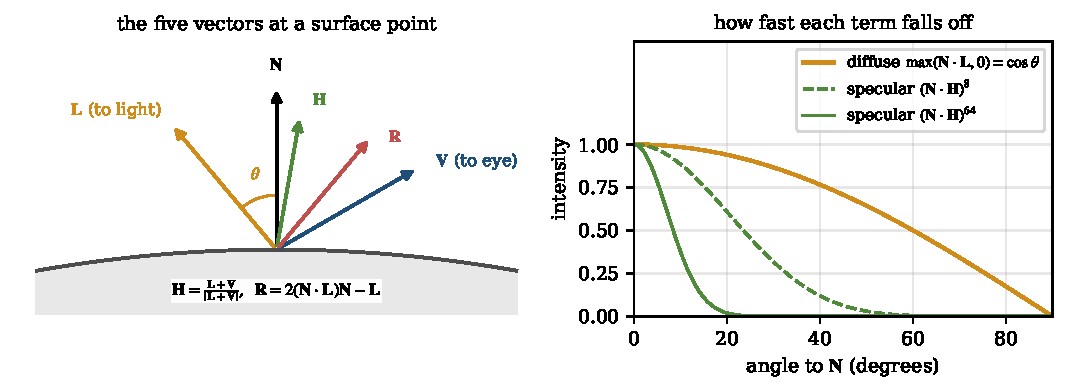
\includegraphics[width=\linewidth]{figures/diagrams/d_lighting.pdf}
\caption{The vectors of Eq.~\ref{eq:phong} at one surface point, and how quickly the diffuse and specular terms fall off with angle (a larger exponent gives a smaller, sharper highlight).}
\label{fig:d-light}
\end{figure}

\begin{figure}[htbp]
\centering
\begin{subfigure}{0.245\linewidth}\raw{scene/v10_light_all}{\linewidth}\caption{All terms.}\end{subfigure}\hfill
\begin{subfigure}{0.245\linewidth}\raw{scene/v10_light_ambient}{\linewidth}\caption{Ambient only.}\end{subfigure}\hfill
\begin{subfigure}{0.245\linewidth}\raw{scene/v10_light_diffuse}{\linewidth}\caption{Diffuse only.}\end{subfigure}\hfill
\begin{subfigure}{0.245\linewidth}\raw{scene/v10_light_specular}{\linewidth}\caption{Specular only.}\end{subfigure}
\caption{The terms of Eq.~\eqref{eq:phong} one at a time on the ammunition bunker at 10:30 (\key{Ctrl+L}).}
\label{fig:terms}
\end{figure}
\begin{figure}[htbp]
\centering
{\footnotesize\textit{Geometry: sun, moon and searchlight at one roof point}}\\[0.5mm]
\wbblock{Illumination}{geometry}\\[2mm]
{\footnotesize\textit{Per-channel ambient, diffuse and specular terms}}\\[0.5mm]
\wbblock{Illumination}{terms}\\[1mm]
{\footnotesize\wbkey}
\caption{Workbook sheet \code{Illumination}: the
three terms for one roof point at noon, sunset, under the moon and under a UAV searchlight. \fullsheet{Illumination}}
\label{fig:wb-illum}
\end{figure}

Ambient light (Figure~\ref{fig:terms}b) has no direction, so the shape reads only through colour. The diffuse term
(c) depends on $\vect N\cdot\vect L$ and darkens faces turned from the sun. The specular term (d) is small, sits on
edges and rims, and moves with the camera because $\vect H$ depends on $\vect V$.
\begin{figure}[htbp]
\centering\plot{p_specular_falloff}{0.62\linewidth}
\caption{The specular lobe $(\vect N\cdot\vect H)^n$ for the shininess values of the scene (2 to 64); $n=64$ gives a
highlight eight times narrower than $n=2$.}
\label{fig:spec}
\end{figure}


In the HDR pipeline (the default) the renderer uses the GGX / Cook--Torrance model of Eq.~\eqref{eq:ggx}; \key{B}
switches to the Blinn--Phong of Eq.~\eqref{eq:phong}, which the display-referred path (\key{N}) always uses.

\subsection{Shadows}
\label{sec:shadows}
A point is lit by the key light (sun or moon) or the searchlight when nothing lies between them. The renderer draws the
scene's depth from each light into a shadow map, then compares depths (Williams' shadow mapping):
\begin{gather}
\vect q=P_lV_l\big(\vect p+\vect N\,t\,(1+2(1-\vect N\cdot\vect L))\big),\qquad (s_u,s_v,z_{\text{ref}})=\tfrac12\,\frac{\vect q_{xyz}}{q_w}+\tfrac12\label{eq:shadow}\\
v=\frac1n\sum_{i=1}^{n}\Big[z_{\text{ref}}-b\le z_{\text{map}}\Big((s_u,s_v)+R_\phi\,\vect o_i\,\frac{\rho}{S}\Big)\Big]\nonumber\\
\text{PCSS: }\ \bar z_b=\operatorname{mean}\{z_{\text{map}}<z_{\text{ref}}\},\qquad
w=(z_{\text{ref}}-\bar z_b)\,\Delta_z\cdot2\tan\tfrac{\theta_s}{2},\qquad \rho=\operatorname{clamp}\big(\tfrac{w}{2t},\rho_0,40\big)\nonumber
\end{gather}
\begin{itemize}
\item $P_lV_l$: the light's view-projection (orthographic cascade for the sun and moon, perspective for the searchlight,
Table~\ref{tab:projs}); $t$: one shadow texel in metres; $b=0.0004$ (cascades), $0.00015$ (searchlight).
\item PCF: $n=8$ or 16 Poisson taps $\vect o_i$ in a disc of $\rho_0=1.6$ texels (near cascade), rotated by a per-pixel
angle $\phi$; each tap is itself a hardware $2\times2$ bilinear compare. $S$ is the map size.
\item PCSS (HIGH and above): the blocker search averages the depths nearer than the receiver, the gap $z_{\text{ref}}-\bar z_b$
(times $\Delta_z$, metres per depth unit) and the light's angular size $\theta_s$ ($1.6^\circ$ sun, $0.53^\circ$ moon) give
the penumbra width $w$; the PCF radius follows it, hard at contact and soft further away.
\item Two cascades cross-fade over the last 20\,\% of the split distance; the key light's visibility is the shadow map
times the cloud shadow times the screen-space contact shadow.
\end{itemize}
\begin{figure}[htbp]
\centering\plot{p_shadows}{\linewidth}
\caption{Shadow filtering with the code's constants: (a) the 16 Poisson taps of \code{kPoisson} at radius 1.6 texels;
(b) the PCSS penumbra width against the blocker gap (Eq.~\eqref{eq:shadow}); (c) the normal-offset bias for the two
EPIC cascades (4096 maps).}
\label{fig:shadowplots}
\end{figure}
\begin{figure}[htbp]
\centering\raw{lab/explorer_stage_08_shadow}{0.85\linewidth}
\caption{Frame Explorer shadow stage: the scene drawn from the light into the depth map (inset) and the lit fraction
per pixel after the PCF of Eq.~\eqref{eq:shadow}.}
\label{fig:shadowstage}
\end{figure}
\begin{table}[htbp]
\caption{Shadow settings per quality preset (\code{RendererFrame.cpp: qualityProfile}).}\label{tab:shadowq}
\centering\small
\begin{tabular}{@{}lllll@{}}
\toprule
 & LOW & HIGH & ULTRA & EPIC\\\midrule
Key-light map (2 cascades) & 1024 & 2048 & 4096 & 4096\\
Searchlight map & off & 1024 & 2048 & 2048\\
Near cascade covers & 10\,m & 12\,m & 14\,m & 14\,m\\
PCF taps $n$ & 8 & 8 & 16 & 16\\
PCSS blocker taps & -- & 8 & 16 & 16\\
Contact-shadow steps & -- & 10 & 12 & 16\\
\bottomrule
\end{tabular}
\end{table}
\begin{lstlisting}[language=C++,caption={The PCF loop of one cascade (\code{ShaderSources.cpp: cascadeShadow}, GLSL).}]
vec4 lp = vp * vec4(P + N * texel * (1.0 + 2.0 * slope), 1.0);   // normal-offset bias
vec3 p = lp.xyz / lp.w * 0.5 + 0.5;                              // light NDC -> [0,1]
float zr = p.z - 0.0004;
float sum = 0.0;
for (int i = 0; i < 16; ++i) {
    if (i >= uPcfTaps) break;
    vec2 o = rot * kPoisson[i] * radius / size;
    sum += texture(uMoonShadow, vec4(p.xy + o, float(layer), zr));   // hardware compare
}
return sum / float(uPcfTaps);
\end{lstlisting}

\textbf{Limitation.} The term split (\key{Ctrl+L}) covers the scene-object and terrain shaders only; grass and
foliage have their own shaders and always show all terms. Practical lamps cast no shadows: only the key light and one
searchlight have shadow maps.
